\documentclass[10pt]{amsart}
\usepackage[a4paper,margin=23mm]{geometry}
\usepackage{amsmath,amssymb,amsthm,mathtools,hyperref,graphicx,xspace,letltxmacro,xpatch}
\usepackage[english]{babel}
\newtheorem{theo}{Theorem}[section]
\newtheorem{lemm}[theo]{Lemma}\newtheorem{prop}[theo]{Proposition}\newtheorem{coro}[theo]{Corollary}\newtheorem{conj}[theo]{Conjecture}
\theoremstyle{definition}\newtheorem{defi}[theo]{Definition}\newtheorem{rema}[theo]{Remark}\newtheorem{exam}[theo]{Example}\newtheorem{exem}[theo]{Example}\newtheorem{nota}[theo]{Notation}
\newcommand{\ie}{i.e.}\newcommand{\eg}{e.g.}\newcommand{\resp}{resp.}\newcommand{\skpt}{\par\smallskip\noindent}
\emergencystretch=3em\pagestyle{plain}
%~Mouliné par MaN_auto v.0.40.4 (569efd63) 2026-04-09 10:14:10


\usepackage{amssymb}
\usepackage{graphicx}

\newcommand{\noopsort}[1]{}
%\renewcommand{\JR}{jun.}

\newcommand{\R}{\mathbb{R}}
\newcommand{\Ss}{\mathbb{S}}
\newcommand{\Z}{\mathbb{Z}}
\newcommand{\C}{\mathbb{C}}
\newcommand{\N}{\mathbb{N}}
\newcommand{\Hh}{\mathbb{H}}

\newcommand{\fkG}{\mathfrak{G}}

\DeclareMathOperator{\II}{II}
\DeclareMathOperator{\Diag}{Diag}
\DeclareMathOperator{\intt}{int}
\DeclareMathOperator{\dist}{dist}
\DeclareMathOperator{\SO}{SO}
\DeclareMathOperator{\PSL}{PSL}
\DeclareMathOperator{\SM}{SM}
\DeclareMathOperator{\SN}{SN}

\theoremstyle{plain}
\newtheorem{probl}{Problem}
\renewcommand*\theprobl{\Alph{probl}}
%%%%%%%%%%%%%%%%%%%%%%%%%%%%%%%%%%%%%%%%%%%%%%%%%%%%%%%%%%%%%%%%%%%%%%%%%%%%%%%%%%%%%%%%%%%%%%%%%%%%%%%%%%%%%%%%%%%%%%%%%%

\graphicspath{{./figures/}}

\newcommand*{\mk}{\mkern -1mu}
\newcommand*{\Mk}{\mkern -2mu}
\newcommand*{\mK}{\mkern 1mu}
\newcommand*{\MK}{\mkern 2mu}

\hypersetup{urlcolor=purple, linkcolor=blue, citecolor=red}

\newcommand*{\relabel}{\renewcommand{\labelenumi}{(\theenumi)}}
\newcommand*{\romanenumi}{\renewcommand*{\theenumi}{\roman{enumi}}\relabel}
\newcommand*{\Romanenumi}{\renewcommand*{\theenumi}{\Roman{enumi}}\relabel}
\newcommand*{\alphenumi}{\renewcommand*{\theenumi}{\alph{enumi}}\relabel}
\newcommand*{\Alphenumi}{\renewcommand*{\theenumi}{\Alph{enumi}}\relabel}
\let\oldtilde\tilde
\renewcommand*{\tilde}[1]{\mathchoice{\widetilde{#1}}{\widetilde{#1}}{\oldtilde{#1}}{\oldtilde{#1}}}
%%%%%%%%%%%%%%%%%%%%%%%%%%%%%%%%%%%%%%%%%%%%%%%%%%
%Better widebar

\makeatletter
\let\save@mathaccent\mathaccent
\newcommand*\if@single[3]{%
  \setbox0\hbox{${\mathaccent"0362{#1}}^H$}%
  \setbox2\hbox{${\mathaccent"0362{\kern0pt#1}}^H$}%
  \ifdim\ht0=\ht2 #3\else #2\fi
  }
%The bar will be moved to the right by a half of \macc@kerna, which is computed by amsmath:
\newcommand*\rel@kern[1]{\kern#1\dimexpr\macc@kerna}
%If there's a superscript following the bar, then no negative kern may follow the bar;
%an additional {} makes sure that the superscript is high enough in this case:
\newcommand*\widebar[1]{\@ifnextchar^{{\wide@bar{#1}{0}}}{\wide@bar{#1}{1}}}
%Use a separate algorithm for single symbols:
\newcommand*\wide@bar[2]{\if@single{#1}{\wide@bar@{#1}{#2}{1}}{\wide@bar@{#1}{#2}{2}}}
\newcommand*\wide@bar@[3]{%
  \begingroup
  \def\mathaccent##1##2{%
%Enable nesting of accents:
    \let\mathaccent\save@mathaccent
%If there's more than a single symbol, use the first character instead (see below):
    \if#32 \let\macc@nucleus\first@char \fi
%Determine the italic correction:
    \setbox\z@\hbox{$\macc@style{\macc@nucleus}_{}$}%
    \setbox\tw@\hbox{$\macc@style{\macc@nucleus}{}_{}$}%
    \dimen@\wd\tw@
    \advance\dimen@-\wd\z@
%Now \dimen@ is the italic correction of the symbol.
    \divide\dimen@ 3
    \@tempdima\wd\tw@
    \advance\@tempdima-\scriptspace
%Now \@tempdima is the width of the symbol.
    \divide\@tempdima 10
    \advance\dimen@-\@tempdima
%Now \dimen@ = (italic correction / 3) - (Breite / 10)
    \ifdim\dimen@>\z@ \dimen@0pt\fi
%The bar will be shortened in the case \dimen@<0 !
    \rel@kern{0.6}\kern-\dimen@
    \if#31
      \overline{\rel@kern{-0.6}\kern\dimen@\macc@nucleus\rel@kern{0.4}\kern\dimen@}%
      \advance\dimen@0.4\dimexpr\macc@kerna
%Place the combined final kern (-\dimen@) if it is >0 or if a superscript follows:
      \let\final@kern#2%
      \ifdim\dimen@<\z@ \let\final@kern1\fi
      \if\final@kern1 \kern-\dimen@\fi
    \else
      \overline{\rel@kern{-0.6}\kern\dimen@#1}%
    \fi
  }%
  \macc@depth\@ne
  \let\math@bgroup\@empty \let\math@egroup\macc@set@skewchar
  \mathsurround\z@ \frozen@everymath{\mathgroup\macc@group\relax}%
  \macc@set@skewchar\relax
  \let\mathaccentV\macc@nested@a
%The following initialises \macc@kerna and calls \mathaccent:
  \if#31
    \macc@nested@a\relax111{#1}%
  \else
%If the argument consists of more than one symbol, and if the first token is
%a letter, use that letter for the computations:
    \def\gobble@till@marker##1\endmarker{}%
    \futurelet\first@char\gobble@till@marker#1\endmarker
    \ifcat\noexpand\first@char A\else
      \def\first@char{}%
    \fi
    \macc@nested@a\relax111{\first@char}%
  \fi
  \endgroup
}
\makeatother

\let\oldbar\bar
\renewcommand*{\bar}[1]{{\mathchoice{\widebar{#1}}{\widebar{#1}}{\widebar{#1}}{\oldbar{#1}}}}
%%%%%%%%%%%%%%%%%%%%%%%%%%%%%%%%%%%%%%%%%%%%%%%%%%%%
\renewcommand*{\to}{\mathchoice{\longrightarrow}{\rightarrow}{\rightarrow}{\rightarrow}}

\newcommand{\longhookrightarrow}{\lhook\joinrel\longrightarrow}
\newcommand*{\hookto}{\mathchoice{\longhookrightarrow}{\hookrightarrow}{\hookrightarrow}{\hookrightarrow}}
%%%%%%%%%%%%%%%%%%%%%%%%%%%%%%%%%%%%%%%%%%%%%%%%%%%%%%%%%%%%%%%%%%%%%%%%%%%%%%

\title{Closed Anosov extension for oriented three-manifolds with boundary}
\author{Guedes Bonthonneau, Yannick}
\date{doi:10.5802/ahl.267; CC BY 4.0}
\begin{document}
\maketitle
\noindent\textit{Editorial note.} Complete original author mathematical body and publisher bibliography retained. Two absent figure overlay TeX files rendered through complete original printed vector diagrams with original labels, excluding captions. Original TeX/PDF unchanged. Standard cited topology inputs remain cited.\par\medskip
\noindent\textit{Allowed standard prerequisites (editorial).}\begin{itemize}
\item Standard functional analysis, measure theory and the author-cited classical theorems. Standard prior results stay cited; complete source-local proofs and definitions retained.
\end{itemize}\medskip


\section{Introduction}

In all that follows, $(M,g)$ will denote a smooth compact Riemannian manifold of dimension $n$, with smooth boundary $\partial M$ and unit tangent bundle $\SM$. The geodesic flow is defined on a subset of $\SM \times\R$, and we will always assume that the trapped set, i.e the set of points $v\in \SM$ whose geodesic trajectory never encounters $\partial \SM$, is a hyperbolic set. As in~\cite{Chen-Erchenko-Gogolev}, we consider the following.

\begin{probl}
\label{probA}
Can $\mathring{M}$ be isometrically embedded as an open set of a compact manifold $(N,g')$ without boundary, so that the geodesic flow of $N$ is Anosov?
\end{probl}

This problem is strongly linked to boundary rigidity, and as the recent article~\cite{Erchenko-Lefeuvre} demonstrates, is crucial in making a link with the marked length spectrum problem. We refer to the introductions of~\cite{Chen-Erchenko-Gogolev,Erchenko-Lefeuvre} for detailed discussions of these important implications. In what follows, we will be implicitly considering embeddings as open sets, i.e isometric \emph{extensions}; if $N$ is allowed to have larger dimension than~$M$, the question is radically different.


Since metrics whose geodesic flow is Anosov do not have conjugate points~\cite{Klingenberg-1974}, certainly $M$ must not have any conjugate point, so we will make this assumption from now on.

It is a standard assumption in the context of inverse problems for manifolds with boundary that the boundary is strictly convex, i.e that the second fundamental form (with respect to the inner pointing normal) satisfies
\begin{equation}\label{eq:convex-boundary}
\II_{\partial M} > 0.
\end{equation}
This implies that $M$ is strictly geodesically convex, and that the behaviour of the geodesic flow near the boundary is quite simple. Without this condition, the problem becomes formidable, and as far as the author is aware, no result is known. We will thus assume~\eqref{eq:convex-boundary}.

\begin{defi}
Let $M$ be a compact manifold with non empty boundary, with hyperbolic trapped set, no conjugate points, and strictly convex boundary. We say that it is \emph{an Anosov manifold with boundary}.
\end{defi}

Let us recall the main result of~\cite{Chen-Erchenko-Gogolev}

\begin{theo}[{\cite[Theorem~A]{Chen-Erchenko-Gogolev}}]
\label{thm:1}
Let $M$ be an Anosov manifold with boundary, and assume that the boundary components of $M$ are topological spheres, then Problem~\ref{probA} has a positive solution.
\end{theo}

Since the only connected compact manifold in one dimension is a sphere, this theorem in particular solves completely the case of surfaces.

In higher dimension, the assumption that the boundary components are spheres seems very stringent, the question being whether there exists any example where $M$ is not a topological ball. In the published version of their paper, the authors in~\cite{Chen-Erchenko-Gogolev} sketch a generalization their argument to the case $\partial M \simeq \Ss^1 \times \Ss^{n-2}$ (see last remark before Section~1.1 therein).

The arguments of~\cite{Chen-Erchenko-Gogolev} were divided into three parts. The first was to observe that when boundaries are spheres, one can always find a manifold with concave boundary, and constant curvature $-1$ that could play the role of $N\setminus M$. In the second one, they constructed an extension of the metric of $M$ on a collar near the boundary, that could be glued with a constant curvature metric. In the last part, using a delicate analysis of Jacobi fields, they obtained hyperbolicity of the geodesic flow of the whole closed manifold.

In this paper, we will give a more general version of the second step in~\cite{Chen-Erchenko-Gogolev}, and discuss at length the first step. We will also observe that the arguments in the third step are quite robust, and extend generally.

Our statement that extends~\cite[Step~2]{Chen-Erchenko-Gogolev} to a more abstract setting is the following

\begin{theo}\label{thm:conformally-compact}
Let $M$ be an Anosov manifold with boundary. Then one can embed isometrically $M\subset N$ into a conformally compact complete manifold $N$ whose interior has uniformly hyperbolic geodesic flow and no conjugate points. The sectional curvature of $N$ is negative outside of a compact set, and tends to a (negative) constant at infinity. Also, $N$ is $M$ with a collar neighbourhood attached to its boundary.
\end{theo}

Here by conformally compact, we mean that the ends of $N$ take the form $(0,1)\times P$, for some compact manifold $P$, and one can find a smooth proper function $f\geq 1$ on $N$, so that compactifying $N$ into $\bar{N}$ by adding to each end $\{1\}\times P$, the metric $(1/f)g_N$ extends smoothly to $\bar{N}$, turning it into a Riemannian manifold with boundary.

Let us now turn to our main result concerning~\cite[Step~1]{Chen-Erchenko-Gogolev}. We prove that, indeed, as suspected by several colleagues when~\cite{Chen-Erchenko-Gogolev} first appeared as a preprint, simple topology of the boundary is a great constraint on the global geometry of $M$.

\begin{theo}\label{thm:special-cases}
Let $M$ be an Anosov manifold with boundary of dimension $n$ at least $3$:
\begin{enumerate}
\item\label{theo1.5.1} If at least one boundary component is diffeomorphic to a sphere, then $M$ is diffeomorphic to a ball, and has no trapped set.
\item\label{theo1.5.2} If at least one boundary component is diffeomorphic to a $\Ss^{n-2}$ bundle over $\Ss^1$, then either the bundle is trivial, and $M$ is diffeomorphic to a solid torus or it is non oriented, and $M$ is diffeomorphic to the product of a M\"obius band and a disk. In both cases, it is a convex neighbourhood of a single closed geodesic.
\end{enumerate}
\end{theo}

As observed by the authors of~\cite{Chen-Erchenko-Gogolev}, in the second case, one can use the residual finiteness of the $\pi_1$ of hyperbolic manifolds to embed $M$ in the finite cover of any given compact hyperbolic $n$-manifold. If one component of the boundary is a $\Ss^{n-p-1}$ bundle over a $p$-dimensional Anosov manifold, one could imagine that $M$ is diffeomorphic to the corresponding ball bundle; except from some partial results, whether this is true or not has eluded the author.

Finally, we show that for 3 manifolds, the problem can also be completely solved.


\begin{theo}\label{thm:3D}
Let $M$ be an oriented Anosov 3-manifold with boundary. Then Problem~\ref{probA} has a positive answer.
\end{theo}


We also obtain:
\begin{coro}\label{cor:1}
If $(M,g)$ is an oriented Anosov 3-manifold with boundary, then there exists a metric $g'$ on $M$ with curvature $-1$ such that $(M,g')$ also has strictly convex boundary (and is thus Anosov with boundary), and is a neighbourhood of the convex core\footnote{The convex core of a convex co-compact manifold is the geodesic convex hull of its closed geodesics.} of a convex co-compact quotient of $\Hh^3$.
\end{coro}

If $(N,g)$ is a convex co-compact 3-manifold whose convex core admits a neighbourhood $V$ that has totally geodesic boundary, one can remove the complement of $V$, and take the double of $V$ along its boundary, to obtain a compact manifold with curvature $-1$ that has the convex core of $N$ as a subset. However, there exist convex co-compact 3-manifold for which one cannot find such a $V$, even modifying the metric. For example, the quotient $N=\PSL_2(\C)/\Gamma$, where $\Gamma$ is a Schottky group, is the interior of a handlebody, and the double\footnote{To obtain a manifold with negative curvature, one has to glue along the boundary with a map that reverses orientation, not the identity.} of a handlebody does not support a metric of curvature $-1$.

It seems that current knowledge of topology of Riemannian manifolds of dimension $\geq 4$ is not sufficient to settle the question in higher dimensions. In particular, since there exist compact manifolds of dimension $\geq 4$, that admit negatively curved metrics, but do not admit a structure of homogeneous space, there can be no equivalent of Corollary~\ref{cor:1} in higher dimension.

\subsection*{Structure of the arguments} 

We will rely on a good part of the argument in~\cite{Chen-Erchenko-Gogolev}. Let us recall the gist of it. The authors first construct an extension of the metric near the boundary, whose curvature is bounded above uniformly, but becomes arbitrarily negative at an arbitrarily small distance of the boundary, and constant at a fixed distance.


\begin{figure}[!h]
\def\svgwidth{0.5\columnwidth}
\centering
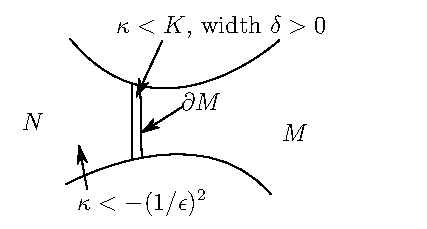
\includegraphics[width=205bp]{boundary-extension-complete.pdf}
%\input{Curvatures-near-boundary-Chen-Erchenko-Gogolev.pdf}
\caption{The extension of the metric near the boundary.}
\end{figure}

The second part is to study the dynamics of Jacobi fields, and prove that the passage of the geodesics through the patch of possibly positive curvature is compensated by the large negative curvature in the rest of the extension and the substantial time spent in that good region. Thus, the extended metric has no conjugate points, and keeps the Axiom A property.

The last part is to find a manifold of constant sectional curvature that can be glued to the extended manifold.

We point out that in the arguments of the second part, it is not really important that the curvature becomes constant far from the boundary. What is crucial is that it is arbitrarily negative on the complement of an arbitrarily small patch near $\partial M$, and uniformly bounded above. If one were to build an extension satisfying only these two properties, the second part of the arguments would apply. Then if one glues to the extension a manifold with concave boundary and negative curvature, the rest of the arguments also apply. The remaining topological question is thus whether there exist concave manifold with negative curvature and prescribed metric near boundary components.

This observation may be relevant in higher dimension. Indeed, starting from dimension~4, there exist manifolds supporting negatively curved metrics, but supporting no locally symmetric metric.

\subsection*{Organization of the paper}

We will first give a slightly different presentation of the construction of the metric extension, so that it applies to the most general case and prove Theorem~\ref{thm:conformally-compact} in Section~\ref{sec:metric-extension}. Next, we will discuss some topological results about the general problem, and finish the proof of Theorem~\ref{thm:special-cases} in Section~\ref{sec:gen-obs-topo}. Finally, we will concentrate on the 3 dimensional case, and prove Theorem~\ref{thm:3D} in Section~\ref{sec:3mfd}.

\subsection*{Acknowledgments}

We happily thank C.~Lecuire for providing the key argument for Theorem~\ref{thm:3D}. We also warmly thank B.~Petri, A.~Erchenko and F.~Paulin for many explanations.


\section{The extension problem}
\label{sec:metric-extension}

We will here present the constructive arguments of~\cite{Chen-Erchenko-Gogolev} a little differently. We start by giving formul\ae\ for the curvatures of a metric in coordinates adapted to a~hypersurface.

\subsection{Study of the curvatures in a slice situation}

In this section, we consider $S$ a compact manifold endowed with a family of Riemannian metrics $(g_t)_t$, and a positive function $f$ of the parameter $t$, that we will assume to lie in an interval $I\subset \R$. Both are assumed to be smooth, and we are chiefly interested in the sectional curvatures of the metrics on $I\times S$ given by
\begin{equation}\label{eq:conformal-slice}
h= dt^2 + g_t,\qquad \tilde{h} = dt^2 + f(t)^2 g_t.
\end{equation}
In what follows, we will think of $g_t$ as fixed, and will let $f$ vary to obtain some interesting properties. Quantities related to $\tilde{h}$ will be denoted with a tilde. In~\cite{Chen-Erchenko-Gogolev}, some very classical formul\ae\ are recalled, but some computations have only been done in local coordinates using Christoffel coefficients; we will here try to give an intrinsic presentation, simplifying the proof of the first part of their statement.

On the manifold $I\times S$, we denote by $T$ the vector field $\partial/\partial t$, and the letters $X,Y$ will denote vector fields tangent to $S$, that do not depend on $t$. From $\|T\|=1$, $[X,T]=0$ and the fact that the Levi--Civita connection has no torsion, we obtain
\[
\nabla_T T = 0.
\]
We also recall that the second fundamental form of the slice $\{t\}\times S$ with respect to $-T$ is
\[
\II = h(\nabla_X T, Y) =\frac{1}{2}\bigl(h(\nabla_T X, Y) + h(X, \nabla_T Y)\bigr) = \frac{1}{2}\partial_t h(X,Y).
\]
(here we used that $\II$ is symmetric, and $\nabla$ torsion free). The shape operator $A$ is defined by
\[
h(AX,Y) = \II(X,Y).
\]
In the following arguments, we will see $A$ as an (operator valued) function of time~$t$, and $A'=\partial_t A = \nabla_T A$ will naturally denote its differential with respect to time. Applying the formul\ae\ above to $\tilde{h}$, we get by definition
\[
f^2 g_t(\tilde{A} X,Y) = \tilde{h}(\tilde{A}X,Y)= \frac{1}{2} \frac{d}{dt}\left[f(t)^2 g_t(X,Y) \right].
\]
so that
\begin{equation}\label{eq:tildeA}
\tilde{A} = \frac{f'}{f} + A.
\end{equation}
We will assume that the slices $S_t =\{t\} \times S$ are strictly convex, i.e that $\tilde{A} > 0$. More precisely, we will assume that $A\geq 0$, and that $f'/f > 0$. We say that the slices are \emph{uniformly} strictly convex if we have $\tilde{A}> C >0$ for some global constant $C>0$.

By $\sigma_{U,V}$, we denote the plane generated by vectors $U,V$. By $R$ we denote the Riemann curvature tensor, by $K$ the sectional curvature, and by $K^{\intt}$ the intrinsic sectional curvature of the slices.

\begin{prop}\label{prop:gauss-codazzi}
We have the following formul\ae\ for the sectional curvatures of $\tilde{h}$, where $a\neq 0$, and $X,Y$ are vector fields on $S_t=\{t\}\times S$, orthonormal for $g_t$ at the point of computation
\begin{align*}
\tilde{K}(\sigma_{X,T}) &= -\frac{f''}{f} + K(\sigma_{X,T}) - 2 \frac{f'}{f} g_t(AX,X). \\
\tilde{K}(\sigma_{X,Y}) &= \frac{1}{f^2} K^{\intt}(\sigma_{X,Y}) + \left[g_t(AX,Y)^2 - g_t(AX,X)g_t(AY,Y)\right] \\
&\quad - \left(\frac{f'}{f}\right)^2 - 2 \frac{f'}{f}\left[g_t(AX,X)+ g_t(AY,Y)\right]\\
\tilde{K}(\sigma_{X+aT,Y})&= \frac{ f(t)^2 \tilde{K}(\sigma_{X,Y}) + a^2 \tilde{K}(\sigma_{T,Y}) + 2a h(R(X,Y)Y,T)}{f(t)^2 + a^2}.
\end{align*}
\end{prop}

\begin{proof}
The main tool here are Gauss' and Codazzi's equations (see~\cite[Section~6.3]{DoCarmo}). In the proof we will not outright assume that $X$ and $Y$ are orthonormal, but rather only perpendicular, because orthonormality changes between $h$ and $\tilde{h}$ (see~\eqref{eq:conformal-slice} while orthogonality does not.

Let us start with the sectional curvature of the plane $\sigma_{X,T}$ generated by $T$ and $X\neq 0$. We recall the proof of~\cite[Eq.~2.7]{Chen-Erchenko-Gogolev}. Only assuming that $X$ does not depend on $t$, we compute
\begin{align*}
h(R(T,X)X, T) &= h(\nabla_T \nabla_X-\nabla_X \nabla_T X, T) \\
& = T(h(\nabla_X X,T)) + h(\nabla_T X, \nabla_X T) \\
& = h(\nabla_X T, \nabla_X T) - T(II(X,X)) \\
&= - h((A'+A^2)X,X).
\end{align*}
We deduce that
\[
K(\sigma_{X,T}) = \frac{h(R(T,X)X,T)}{g_t(X,X)}= - \frac{g_t((A'+A^2)X,X)}{g_t(X,X)}.
\]
Applying this identity to $\tilde{h}$, and using~\eqref{eq:tildeA}, elementary computations give
\[
\tilde{K}(\sigma_{X,T}) = - \frac{f''}{f} + K(\sigma_{X,T}) - 2 \frac{f'}{f} \frac{g_t(AX,X)}{g_t(X,X)}.
\]


Let us now turn to the curvature of the plane $\sigma_{X,Y}$ generated by $X$ and $Y$. Gauss' equation gives
\[
K(\sigma_{X,Y}) = K^{\intt}(\sigma_{X,Y}) - \frac{ g_t(AX,X)g_t(AY,Y) - g_t(AX,Y)^2}{g_t(X,X)g_t(Y,Y) - g_t(X,Y)^2},
\]
where $K^{\intt}$ is the sectional curvature of $g_t$. Since $f$ is constant on each slice, we find directly
\[
\tilde{K}^{\intt}(\sigma_{X,Y}) = \frac{1}{f^2} K^{\intt}(\sigma_{X,Y}).
\]
Assuming just for this equation that $X$ and $Y$ orthonormal (for $g_t$) at the point of interest, we obtain
\[
\begin{split}
\tilde{K}(\sigma_{X,Y}) &= \frac{1}{f^2} K^{\intt}(\sigma_{X,Y}) - \left[g_t(AX,X)g_t(AY,Y) - g_t(AX,Y)^2\right] \\
&\quad - \left(\frac{f'}{f}\right)^2 - 2 \frac{f'}{f}(g_t(AX,X) + g_t(AY,Y)).
\end{split}
\]

Let us now turn to the curvature of the plane $\sigma_{X+aT,Y}$, generated by $X + aT$ and~$Y$, for some $a\neq 0$. Assuming $X$ is not collinear to $Y$, without changing the plane (but changing $a$), we can assume that $X,Y$ are orthogonal (for $g_t$) at the point of interest. Then we have
\[
K(\sigma_{X+aT, Y}) = \frac{ h(R(X+aT, Y)Y, X+aT)}{(a^2+g_t(X,X))g_t(Y,Y)}.
\]
This gives (using the symmetries of the curvature tensor)
\[
\begin{split}
K(\sigma_{X+aT, Y}) =& \frac{1}{a^2+g_t(X,X)^2}\left(g_t(X,X)^2 K(\sigma_{X,Y}) + a^2 K(\sigma_{T,Y})\right) \\
& + \frac{2a}{(a^2+g_t(X,X)^2)g_t(Y,Y)}h(R(X,Y)Y,T).
\end{split}
\]
It is this last mixed term in the RHS that was estimated using coordinates and Christoffel coefficients in~\cite{Chen-Erchenko-Gogolev}. We are seeking to compute
\[
F(X,Y):= h\left(\nabla_X \nabla_Y Y - \nabla_Y \nabla_X Y - \nabla_{[X,Y]} Y, T\right).
\]
According to the Codazzi equation, we have
\[
F(X,Y)=\nabla_X^{\intt} II(Y,Y) - \nabla_Y^{\intt} II(X,Y).
\]
Now, we observe that
\[
\tilde{F}(X,Y)= f(t)^2 F(X,Y).
\]
This $f(t)^2$ term will be compensated by $\tilde{h}(Y,Y)$, so we conclude that
\[
\tilde{K}(\sigma_{X+aT,Y}) = \frac{ f(t)^2 \tilde{K}(\sigma_{X,Y}) + a^2 \tilde{K}(\sigma_{T,Y}) + 2 a F(X,Y) }{f(t)^2 + a^2}.\qedhere
\]
\end{proof}

\subsection{Extension of the metric}

We assume that we are given $(M,g)$ as in the introduction. Near the boundary, we can always add cylinders, to define
\[
N:= M \cup (\partial M)_x\times\mathopen{]}0, +\infty]_t,
\]
which is a smooth manifold with boundary, diffeomorphic to $M$. Theorem~\ref{thm:conformally-compact} follows from the next lemma.

\begin{lemm}\label{lemma:extension}
We can build a metric $\tilde{h}$ on the interior of $N$ that extends the metric of $M$, such that this metric is conformal to a smooth metric on $N$. Additionally, there exists a constant $C_0>0$ such that for $\kappa>0$ large enough, we can ensure that:
\begin{enumerate}\romanenumi
\item\label{lemm2.2.1} In $\mathring{N}\setminus M$, the sets $\{t=t_0\}$ are equidistant sets from the boundary $\partial M$. They are uniformly strictly convex.
%\pagebreak
\item\label{lemm2.2.2} The sectional curvature of $\tilde{h}$ tends to $-\kappa^2$, with equality for $t\geq 1$ if $\partial M$ supports a constant curvature metric.
\item\label{lemm2.2.3} The sectional curvature of $\tilde{h}$ is globally bounded above by $C_0$.
\item\label{lemm2.2.4} For $t\geq 1/\sqrt{\kappa}$, the sectional curvature of $\tilde{h}$ is less than $-\kappa^2/2$.
\end{enumerate}
\end{lemm}

\begin{proof}
We will work near a fixed boundary component $P\subset \partial M$. Near $P$, we can write the metric in the form
\[
h=dt^2 + g_t(dx),
\]
where $g_t$ is a family of metrics on $P$, $-\epsilon< t\leq 0$, and $t$ is the geodesic distance to $P$. We can extend the family $g_t$ smoothly to $\mathopen{]}-\epsilon, +\infty\mathclose{[}$, and since $\partial_t g_t > 0$ near $ t = 0$, we can ensure that:
\begin{itemize}
\item $\partial_t g_t > \tfrac{1}{2}\partial_t g_t|_{t=0}$ for $t\in\mathopen{]}-\epsilon, 1/2]$,
\item $\partial_t g_t \geq 0$ for all $t$'s,
\item $\partial_t g_t = 0$ for $t\geq 1$.
\end{itemize}
There is great flexibility in the way $g_t$ is constructed; in particular the value of $g_1$ can be chosen almost arbitrarily, up to a dilation factor. We will use this when $P$ supports a metric of constant sectional curvature. If $g'$ is such a metric, and $C_1>0$ is large enough, we can ensure that $g_t = C_1 g'$ for $t\geq 1$. The constant $C_1$ is fixed now and arbitrarily.

Next, we want to look for $\tilde{h} = dt^2 +f(t)^2 g_t(dx)$ in the form given by the previous section. We impose $f=1$ on $\mathopen{]}-\epsilon, 0]$. We will use the conclusions of Proposition~\ref{prop:gauss-codazzi} leisurely.

Let us analyze the conditions of the theorem and their consequence for $f$. First, to ensure uniform strict convexity, it suffices to assume that $f''\geq 0$ globally, and that $f'/f>C>0$ on $[1/2, +\infty\mathclose{[}$. Next, $f''\geq 0$ also ensures\footnote{One needs that $f''\geq 0$, $f'\geq 0$ and $f\geq 1$. Since $f=1$ on $\mathopen{]}-\epsilon, 0]$ and is smooth, it suffices to assume that $f''\geq 0$.} that the sectional curvatures satisfy $\tilde{K}\leq K$, so that~\eqref{lemm2.2.3} is satisfied with $C_0 \geq \sup K$.

Let us now consider~\eqref{lemm2.2.2}. In the domain $t\geq 1$, $\partial_t g_t = 0$ implies
\begin{align*}
\tilde{K}(\sigma_{X,T}) &= -\frac{f''}{f} \\
\tilde{K}(\sigma_{X,Y}) &= \frac{1}{f^2}K^{\intt}(\sigma_{X,Y}) - \left(\frac{f'}{f}\right)^2\\
\tilde{K}(\sigma_{X+aT,Y})&= \frac{ f(t)^2 \tilde{K}(\sigma_{X,Y}) + a^2 \tilde{K}(\sigma_{Y,T})}{f(t)^2+ a^2}.
\end{align*}
This suggests to take $\kappa>0$ and set
\begin{equation}\label{eq:f-away}
f_{cc}(t):=
\begin{cases}
\frac{C}{\kappa} \cosh(\kappa t) & \text{if }\inf K^{\intt}_{t\geq 1} = - C^2<0,\\
e^{\kappa t} &\text{if }K^{\intt}_{t\geq1} =0,\\
\frac{C}{\kappa} \sinh(\kappa t) & \text{if }K^{\intt}_{t\geq 1}\geq 0\quad\text{and}\quad\sup K^{\intt}_{t\geq 1} = C^2 >0.
\end{cases}
\end{equation}
For $t\geq 1$, we take $f= f_{cc}$. This ensures that the curvature tends to $-\kappa^2$ as $t\to+\infty$ (exponentially fast in $t$). When $g_{1}$ has constant curvature, we have $\tilde{K}=-\kappa^2$ for $t\geq 1$.

Now, for~\eqref{lemm2.2.4}, we observe that for $C_2$ large enough, and for $t > 0$,
\begin{align}\label{eq:bound-bis}
\tilde{K}(\sigma_{X,T}) &\leq - \frac{f''}{f} + C_2,\qquad \tilde{K}(\sigma_{X,Y}) \leq \frac{C_2}{f^2} - (f'/f)^2,
\\
\tilde{K}(\sigma_{X+aT,Y}) &\leq \max\left(\tilde{K}(\sigma_{X,T}),\; \tilde{K}(\sigma_{X,Y})\right) + \frac{C_2}{f}.\nonumber
\end{align}
Here in the formula for the curvature of $\sigma_{X+aT,Y}$ from Proposition~\ref{prop:gauss-codazzi}, we have used that $2a/(a^2+f^2)\leq 1/f$. Let $t_0\in(0,1)$ be such that the function $f_{cc}$ defined in~\eqref{eq:f-away} satisfies $f_{cc}\geq 1$ for $t\geq t_0$. This suggests to extend the choice $f=f_{cc}$ to $t\geq t_0$, getting on that range
\begin{equation}\label{eq:bound}
\tilde{K} \leq C_3 - \kappa^2,
\end{equation}
for $C_3$ large enough. Indeed elementary computations show that the worst bound is
\[
\tilde{K} \leq \frac{C_2}{f} + \frac{C_2}{f^2} - (f'/f)^2,
\]
when $f= C \cosh(\kappa t)/\kappa$, and $C_2$ is the constant from~\eqref{eq:bound-bis}. This becomes
\[
\tilde{K} \leq \frac{2C_2}{f} + \frac{\kappa^2}{\cosh(\kappa t)^2} - \kappa^2 = \frac{2C_2}{f} + \frac{C^2}{f^2} - \kappa^2,
\]
So that $C_3= 2C_2 +C^2$ is suitable for~\eqref{eq:bound}. We observe that (for example), $t_0 = 1/\sqrt{\kappa}$ satisfies the condition for $\kappa$ large. We also observe that $f_{cc}''\geq 0$ for $t\geq 0$, and $f_{cc}'/f_{cc}> C>0$ for $t>1/2$, uniformly as $\kappa$ becomes large. It remains thus to define $f$ on the interval $[0,1/\sqrt{\kappa}]$ so that $f''\geq 0$, to obtain a smooth function. The only condition for this is that $(0,f(0))=(0,1)$ is strictly above the tangent to the graph of $f_{cc}$ at $t=t_0 =1/\sqrt{\kappa}$. Accordingly, we require that
\[
f_{cc}(t_0) - f_{cc}'(t_0) t_0 < 1.
\]
We can then check case by case that this holds for $t_0 = 1/\sqrt{\kappa}$ and $\kappa$ large enough.

Let us finally check the smooth conformal compactness. For this, it suffices to set $y = e^{-\kappa t}$, to write the metric in the cylinder in the form
\[
\tilde{h} = \frac{1}{\kappa^2 y^2}\left(dy^2 + m(y)g_1(dx)\right).
\]
Here, the function $m$ is a smooth non-vanishing function of $y^2$, and $y$ is a boundary defining function.
\end{proof}



\section{General observations about the topology of the problem}\label{sec:gen-obs-topo}

Let us recall some facts on universal covers of manifolds with hyperbolic geodesic flow.

We will denote by $\pi:\widetilde{M}\to M$ the universal cover of $M$, and by $\widetilde{N}$ that of $N$. Since $M$ is geodesically convex and does not have conjugate points, we can pick $x_0\in M$ and identify $\widetilde{M}$ with the set of $u\in T_{x_0} M$ such that $\exp_{x_0}(u)\in M\simeq \R^n$. By this construction, we identify $\widetilde{M}$ as a geodesically convex subset of $\widetilde{N}\simeq \R^n$ (according to~\cite{Kobayashi-61}). The fundamental group $\pi_1(M)$ is realized by isometries of $\widetilde{N}$, which preserve $\partial \widetilde{M}$.

The embedding $\imath : \partial M \hookto M$ induces a map $\imath_\ast : \pi_1(\partial M)\to \pi_1(M)$. Let $P$ be a~connected component of $\partial M$, and $\tilde{P}$ be a~connected component of $\pi^{-1}(P)$. Since $\tilde{N}$ is simply connected, the closed curves on $\tilde{P}$ can always be deformed to points in~$\tilde{N}$. This leads to
\[
\pi_1(\tilde{P}) = \{ \gamma \in \pi_1(P)\ |\ \imath_\ast(\gamma) = 0\}.
\]
We deduce that $P = \tilde{P}/\imath_\ast(\pi_1(P))$.

The elements of $\pi_1(M)$ (except $1$) are represented by a special kind of isometries, called \emph{loxodromic}. They have a continuous extension to (H\"older) homeomorphisms of $B^n = \tilde{N}\cup\Ss^{n-1}$ (the \emph{visual compactification} of $\tilde{M}$). They have exactly two fixed points, which lie in $\Ss^{n-1}$. They preserve the corresponding geodesic, along which they are a translation. In particular, if two isometries $\gamma$, $\mu$ commute, there must exist another $\eta$, and $k,\ell\in\N$ so that $\gamma = \eta^k$, $\mu = \eta^\ell$. This implies that there is no copy of $\Z^2$ inside $\pi_1(M)$.

Projecting $\partial \tilde{M}$ along rays from $x_0$ on $\Ss^{n-1}$, we find that $\partial\tilde{M}$ is (H\"older) homeomorphic to an open set of $\Ss^{n-1}$. Its complement $\Lambda$ is called the \emph{limit set}. It is the set of endpoints of geodesics that remain inside in $M$ for all times.

From these general facts, we deduce our Theorem~\ref{thm:special-cases}.

\begin{proof}[{Proof of Theorem~\ref{thm:special-cases}}]
Let us start by observing that the following are equivalent:
\begin{enumerate}
\item\label{prftheo1.5pt1} at least one connected component of $\partial \tilde{M}$ is a sphere.
\item\label{prftheo1.5pt2} At least one connected component of $\partial \tilde{M}$ is compact.
\item\label{prftheo1.5pt3} $\partial\tilde{M}\simeq \Ss^{n-1}$.
\item\label{prftheo1.5pt4} $\tilde{M}\simeq B^n$.
\item\label{prftheo1.5pt5} $\pi_1(M) =\{1\}$.
\item\label{prftheo1.5pt6} $M$ is diffeomorphic to a closed ball.
\end{enumerate}

Certainly, \eqref{prftheo1.5pt1} implies~\eqref{prftheo1.5pt2}, and since $\partial \tilde{M}$ is an open set of $\Ss^{n-1}$, if one of its connected component is compact, it must be the whole sphere, so~\eqref{prftheo1.5pt2} implies~\eqref{prftheo1.5pt3}. Using rays starting from $x_0$, we can then build a diffeomorphism between $\tilde{M}$ and $B^n$, so that~\eqref{prftheo1.5pt3}
implies~\eqref{prftheo1.5pt4}. In that case, every element of $\pi_1(M)$ preserves a compact set of $\R^n$, so must be trivial, and~\eqref{prftheo1.5pt4} implies~\eqref{prftheo1.5pt5}. If~\eqref{prftheo1.5pt5} holds, then $M= \tilde{M}$ must be compact, and using again rays from $x_0$, we find that $M$ is a closed ball. Finally, if $M$ is a closed ball, its boundary is a sphere. This takes care of Theorem~\ref{thm:special-cases}$\MK$\eqref{prftheo1.5pt1}.

For Theorem~\ref{thm:special-cases}$\MK$\ref{theo1.5.2}, we rely on the equivalence between:
\begin{enumerate}\alphenumi
\item\label{prftheo1.5pta} $\Lambda$ has exactly two points.
\item\label{prftheo1.5ptb} $\partial M$ is diffeomorphic to a bundle: $\Ss^{n-2} \to \partial M \to \Ss^{1}$.
\item\label{prftheo1.5ptc} One connected component of $\partial M$ is diffeomorphic to a bundle ${\Ss^{n-2} \to P \to \Ss^{1}}$.
\item\label{prftheo1.5ptd} One connected component $P$ of $\partial M$ satisfies $\imath_\ast(\pi_1(P))\simeq \Z$.
\end{enumerate}

Certainly, \eqref{prftheo1.5pta} implies that $\pi_1(M)$ is generated by a non trivial loxodromic isometry~$\gamma$. It preserves a single geodesic, along which we can take Fermi coordinates. This provides a decomposition of $\tilde{N}$ in the form $\R\times \R^{n-1}$, where $\gamma$ acts as follows:
\[
\gamma(t,x) = (t+\ell_\gamma, A_\gamma x).
\]
Here, $\ell_\gamma$ is the translation length of $\gamma$ and $A_\gamma\in O(n-1)$. The preserved geodesic is given by $\R\times\{0\}$. Since $\gamma$ must be represented in $M$ by a closed geodesic, this implies that $\R \times \{0\} \subset \tilde{M}$. The convexity of $M$ implies that the intersection $\tilde{M}\cap \{t\} \times \R^{n-1}$ is star-shaped for every $t\in\R$. Additionally, since $\pi_1(M) = \langle\gamma\rangle$, this intersection must be compact, with smooth boundary, so that it is diffeomorphic to a ball. We deduce that the boundary of $M$ is diffeomorphic to the sphere bundle
\[
\R \times \Ss^{n-1}/{(t,x)\sim (t+\ell_\gamma, A x)}.
\]
Topologically, there are exactly two such bundles\footnote{Because $\SO(n-1)$ is connected.}: either $A\in \SO(n-1)$, and this is the trivial bundle, or $\det A = -1$, and $M$ is not oriented, with a M\"obius-band like structure. This implies~\eqref{prftheo1.5ptb} (which implies~\eqref{prftheo1.5ptc}).

Let us assume~\eqref{prftheo1.5ptc} and let $P$ be the corresponding connected component, and $\tilde{P}$ a~connected component of $\pi^{-1}(P)$. From the arguments in the ball case above, we know that $\tilde{P}$ cannot be compact. If $n>3$, this implies $\tilde{P} = \R \times \Ss^{n-2}$, and $\imath_\ast(\pi_1(P)) \simeq \Z$ is generated by one non trivial isometry. In the case $n=3$, we have to consider that case $\tilde{P}\simeq \R^2$. However, since $\pi_1(M)$ cannot contain $\Z^2$, this case is ruled out, and so it is the same as $n>3$, and we have~\eqref{prftheo1.5ptd}.

Now, assuming~\eqref{prftheo1.5ptd}, let $\imath_\ast(\pi_1(P))= \langle\gamma\rangle$. Then let $c(t)$ be the geodesic preserved by $\gamma$. We find that $\tilde{P}$ is at bounded distance from $\{c(t) | {t\in\R}\}$. This implies that $\partial \tilde{P}$ (seen as a subset of $\Ss^{n-1}$) can only contain the endpoints of $c(t)$, and so this implies~\eqref{prftheo1.5pta}.
\end{proof}

As we have seen above, the topological type of the boundary constrains the type of a manifold. Let us discuss now some more partial results in this direction.

\begin{lemm}
Let us assume that a boundary component $P$ satisfies $\Gamma:=\imath_\ast(\pi_1(P))= \pi_1(\Sigma)$, where $\Sigma$ is a compact Anosov manifold of dimension $p\leq n-2$. Then $P$ is the only boundary component.
\end{lemm}

\begin{proof}
In that case, the visual boundary $\partial \Gamma$ is homeomorphic to a sphere $\Ss^{p-1}$, and since $\Gamma$ is a hyperbolic subgroup of $\pi_1(M)$, the limit set of $\Gamma$, which must be also $\partial \tilde{P}$, is also homeomorphic to $\Ss^{p-1}$. Since $\Ss^{n-1}\setminus\Ss^{p-1}$ must be connected~\cite[Proposition~2.B.1]{Hatcher}, we deduce that $\Ss^{n-1}\setminus \Ss^{p-1} = \tilde{P}$. This means that $P$ is the whole boundary of $M$.
\end{proof}

If the embedding of $\Ss^{p-1}$ into $\Ss^{n-1}$ is the standard one, we get that $\tilde{P}\simeq \Ss^{n-p-1}\times\R^{p}$, and $M$ turns out to be tubular neighbourhood of $\Sigma$. However, there are more than one way to embed a sphere in another, except in the case that $n> 2p$.

\begin{coro}
If $\Sigma$ is a surface, and $M$ has dimension at least $5$, then $M$ is diffeomorphic to a ball bundle over $\Sigma$.
\end{coro}

In 4 dimensions, understanding exactly which $B_2$ bundles over a compact surface can be endowed with a complete convex hyperbolic structure is not completely solved. This question was investigated by several authors (see~\cite{gromov,convex-plumbing}).


Let us close this section with a modicum of information regarding the general case for the possible shape of the boundary. We specialize to the case of $M$ having 4 dimensions, to be able to use the geometrization theorem. For this, we will rely on several results from the theory of the topology of 3 manifolds. For example, the reader can consult~\cite[Section~3]{Freitas}. Since it is not our main focus, we will be very cursory.

\begin{lemm}
Let $M$ be an orientable Anosov $4$-manifold with boundary, with some boundary component $P\neq \emptyset$. Assume that $P\subset M$ is $\pi_1$-injective. Then either $P=\Ss^3$ or it decomposes as a connected sum
\[
A_1 \#\dots \# A_p \# B_1 \# \dots \# B_\ell,
\]
where each $A_j$ is a copy of $\Ss^2\times \Ss^1$, and each $B_j$ is a compact hyperbolic 3 manifold.
\end{lemm}

\begin{proof}
According to the prime decomposition theorem~\cite{Milnor}, we can decompose
\[
P = P_1 \# \dots \# P_m,
\]
where each $P_j$ is orientable and none can be decomposed as a non-trivial connected sum, and (unless $P= \Ss^3$) each $P_j$ is either $\Ss^1\times\Ss^2$ or is irreducible (i.e every embedding of $\Ss^2$ bounds a ball). According to Van~Kampen's theorem, we have that
\[
\pi_1(P)= \pi_1(P_1)\ast \dots \ast \pi_1(P_m).
\]

According to the geometrization theorem, we can decompose each irreducible\linebreak $P_j$ as
\[
P_j = \cup Q_{j,\ell},
\]
where each $Q_{j,\ell}$ is a manifold whose boundary components are torii (said to be \emph{incompressible}), and whose interior admits a geometric structure, in the list of Thurston's 8 geometries. Also, each torus boundary is $\pi_1$ embedded.

Since we assumed that $P$ is $\pi_1$-injective, and $\pi_1(M)$ cannot contain a $\Z^2$ subgroup, we deduce that there cannot exist any incompressible torus in the boundary, and, in particular, the decomposition of the $P_j$ must be trivial: each of them supports a~Thurston geometry.

Among the Thurston geometries, we observe that for either a compact Euclidean, Nil or Sol manifold, the fundamental group must be a semi-direct product $\Z^2 \times \Z$, which contains a $\Z^2$.

In the $\Hh^2\times\R$ or $\tilde{SL(2,\R)}$ case, the fundamental group must contain a cyclic normal subgroup, i.e a $\Z$ center. Since we cannot have torsion, it must also contain a $\Z^2$, and this is also ruled out.

Next, we observe that in the spherical case, elements of the $\pi_1$ must have finite order, which is not possible because there are no elliptic elements in $\pi_1(M)$. In particular, if $P_j$ has spherical geometry, $P_j = \Ss^3$, so that $P=P_j$.


We deduce that each $P_j$ has geometry either $\Ss^2\times\R$, or $\Hh^3$, or is a sphere. In the first case, since $P_j$ is orientable, it is diffeomorphic to $\Ss^2 \times \Ss^1$. In the second case, $P_j$ is a hyperbolic $3$-manifold.
\end{proof}


\section{The case of 3-manifolds}\label{sec:3mfd}

In this section, let us concentrate on the case that $M$ is 3 dimensional and oriented. Then the boundary components are compact oriented surfaces, so either a sphere, a torus or surfaces of genus $g>1$. As we have seen, if $M$ is neither a solid torus nor a ball, all the components must be of the latter variety. The authors of~\cite{Chen-Erchenko-Gogolev} have already shown how to embed the torus or the ball, so we will concentrate on the remaining case. As noted in Lemma~\ref{lemma:extension}$\MK$\eqref{lemm2.2.2}, we can assume that the boundary components have constant curvature. We can even choose freely the hyperbolic metric on the boundary.

\begin{theo}\label{thm:compact-embedding-geometry}
Let $M$ be a 3-manifold whose boundary is strictly convex, with curvature $-\kappa^2$ constant near the boundary. Assume further that all connected components of the boundary are hyperbolic surfaces of genus $g>1$. Possibly using Lemma~\ref{lemma:extension} to change the hyperbolic structure on the boundary, $M$ can be embedded into a compact manifold $N'$ without boundary, such that the curvature is $-\kappa^2$ in $N'\setminus M$.
\end{theo}

%%
\begin{proof}
We start by recalling the following:

\begin{lemm}[{\cite[Theorem~3.3]{Fujii}}]
\label{lemma:Fujii}
For $g>1$, there exists $N_g$ a compact hyperbolic 3-manifold whose boundary is a totally geodesic surface $S_g$ of genus $g$.
\end{lemm}

(As explained in the introduction of~\cite{Fujii}, not all hyperbolic structures on surfaces can be realized as totally geodesic boundaries, essentially because of Mostow rigidity).

Let us come back to our problem. Without loss of generality, we assume that the boundary of $M$ is connected and denote $\Sigma=\partial M$. If there are several components, one can work componentwise. We endow $\Sigma$ with a hyperbolic metric $g_{\partial N_g}$ so that Lemma~\ref{lemma:Fujii} applies, and we also have $\Sigma = \partial N_g$ as a totally geodesic boundary. Near the boundary of $(N_g, h_0)$, we have
\begin{equation}\label{eq:near-boundary-N_g}
N_g \simeq \Sigma_x \times [0, \delta\mathclose{[}_\tau,\qquad h_0 = d\tau^2 + \cosh(\tau)^2 g_{\partial N_g}(x,dx).
\end{equation}
Let us apply the construction of Section~\ref{sec:metric-extension}. For $C_0>0$ large enough, we can ensure that $C_0 g_{\partial N_g}> g_{\partial M}$, where $g_{\partial M}$ is the metric on $\Sigma\simeq \partial M$. We can thus build an extension $M\subset N$ according to Lemma~\ref{lemma:extension}. In $N\setminus M$, for $1\leq t\leq 2$, the metric takes the form (for some $\kappa>0$)
\[
dt^2 + \frac{1}{\kappa^2}\cosh(\kappa t)^2 g_{\partial N_g}(x,dx).
\]
In the formula above we recognize the expression in coordinates of the metric $h_0/\kappa^2$ (here, $\tau = \kappa t$). If the local coordinates in~\eqref{eq:near-boundary-N_g} extend as far as $\tau \leq 2\kappa$, we can thus glue $N_{\{t< 2\}}$ with $N_g\setminus \Sigma\times[0,2\kappa[$, and this will conclude the proof of Theorem~\ref{thm:compact-embedding-geometry} setting
\[
N' = N_{\{t<2\}}\cup (N_g\setminus \Sigma\times [0,2\kappa\mathclose{[}).
\]
The difficulty here is that for the dynamical arguments of~\cite{Chen-Erchenko-Gogolev} to apply, we need to be able to take $\kappa$ arbitrarily large. We will thus be done if we can prove

\begin{lemm}\label{lemma:good-N_g}
For any $\kappa>0$, we can choose $N_g$ such that the $2\kappa$ neighbourhood of $\partial N_g$ is diffeomorphic to $\partial N_g \times [0,2\kappa\mathclose{[}$.
\end{lemm}

The argument of the proof was communicated by C.~Lecuire. It relies on the following very fine statement from the topology of hyperbolic manifolds

\begin{theo}[{\cite[Theorem~9.2]{Agol2012}}]
Fundamental groups of compact 3 dimensional hyperbolic manifolds are LERF (locally extended residually finite).
\end{theo}

This means that whenever $H\subset \pi_1(M)$ is finitely generated, and $\gamma\in \pi_1(M)\setminus H$, there exists a finite index subgroup $\Gamma\subset\pi_1(M)$ such that $H\subset \Gamma$ and $\gamma\notin \Gamma$.

Let us come back to:

\begin{proof}[Proof of Lemma~\ref{lemma:good-N_g}]
We will build $N_g$ by induction, so we start by denoting $N_g^0$ the one provided by Lemma~\ref{lemma:Fujii}. Let us now consider geodesics of $N_g^0$ with endpoints in its boundary. We will say that two such geodesics are boundary-homotopic, if there is a free homotopy between them, so that at each time, the endpoints remain in the boundary. We claim that any such geodesic is either boundary homotopic to a point in the boundary, or to a geodesic that intersects the boundary orthogonally. Additionally, such a boundary-orthogonal geodesic uniquely minimizes the length among its boundary-homotopy class.

We first prove that any geodesic from the boundary to itself is boundary homotopic to a geodesic that is orthogonal to the boundary at one endpoint. For this we pick a component $P$ of the boundary of the universal cover $\tilde{N_g^0}\subset \Hh_3$. Consider now a~geodesic $\gamma_0$ with endpoints in the boundary. We can lift it to a geodesic $\gamma$ of $\tilde{N_g^0}$ with starting point $x\in P$. Its other endpoint lies in some component $P'=\gamma P$. If $P'= P$, then the original geodesic $\gamma_0$ must actually lie in the boundary of $N_g^0$ and it is boundary homotopic to a point. Now we consider the case $P'\neq P$. Then we can find $y\in P'$ minimizing the distance from $P'$ to $x$. The geodesic from $x$ to $y$ must be orthogonal to $P'$, and projects down on $N_g^0$ to a geodesic orthogonal to the boundary at the second endpoint.

Let $\Omega\subset \partial N_g^0 = \Sigma$ be the set of points $x$ for which the geodesic $\gamma_x$ starting from $x$ orthogonally to $\Sigma$ eventually reaches $\Sigma$ again. Its connected components correspond exactly to boundary homotopy classes of corresponding geodesics. Let us denote by~$U$ such a connected component. The length of the geodesic $\gamma_x$ as $x\in U$ approaches the boundary of $U$ must tend to $+\infty$, so that there exists in $U$ a point $x$ with $\gamma_x$ minimizing the length in the corresponding boundary homotopy class. For such a~point, elementary arguments show that the geodesic must be orthogonal at \emph{both} endpoints.

For uniqueness, observe that if we have two points $x,x'$ in $P$, with corresponding two endpoints $y,y'$ in $P'$, we can form the quadrilateral $xx'y'y$, which is contained in a copy of $\Hh_2$ in $\Hh_3$, and has all right angles. This is not possible unless its area is zero, so that two sides coincide, i.e $x=x'$.

Let us set
\[
\fkG(N_g^0)= \{ a \mid \text{some boundary-orthogonal geodesic has length $a$.} \}
\]
Certainly, $\fkG(N_g^0)$ is a discrete set, and its only accumulation point is $+\infty$. We can enumerate it as
\[
\fkG(N_g^0)= \{ 2 \ell_j \mid j\geq 0\}.
\]

With a bit more of elementary Riemannian geometry, we find that $\ell_0$, the largest $\ell$ such that the $\ell$-neighbourhood of $\Sigma$ is product, is exactly half the length of a shortest boundary-orthogonal geodesic (there may be several non-boundary homotopic orthogonal geodesics with the same length).


Let us denote $m_0>0$ the number of boundary-orthogonal geodesics with length $2\ell_0$, and $\gamma_0$ one of them. Let us now consider the double $A_0 = DN_g^0$ of $N_g^0$ (i.e two copies of $N_g^0$ glued along their boundaries $\Sigma$), and $D\gamma_0$ the double of $\gamma_0$, a closed geodesic of length $4\ell_0$. Using the LERF theorem, we find a finite index subgroup $\Gamma\subset \pi_1(A_0)$ so that $\pi_1(\Sigma) \subset \Gamma$, and $[D\gamma_0]\notin \Gamma$. Let us denote $B_0 = \Hh^3/\Gamma$ the corresponding cover of $A_0$.

The condition $\pi_1(\Sigma)\subset \Gamma$ ensures that the preimage of $\Sigma$ by the covering map is a finite disjoint union of copies of $\Sigma$. Removing them from $B_0$, we obtain a finite collection of connected open set whose closures we denote by $T_j$. Each of them is a~hyperbolic 3 manifold with boundary, finitely covering $N_g^0$.

Among the $T_j$'s, at least one of them has more than one boundary component, otherwise we would have $B_0 = A_0$. For every $T_j$, we can consider the lifts of $\gamma_0$ to $T_j$, and, in particular, the ones that have endpoints in different boundary components. If there were no such lift, $D\gamma_0$ would be lifted to $B_0$ as a closed geodesic, which would be a contradiction with the choice of cover. Thus we can find at least one $T_{j_0}$, and one lift of $\gamma_0$, which starts from some boundary component $\Sigma_0 \simeq \Sigma$ and ends in a different boundary component. Let us consider $N_g^{0,1}$ the manifold obtained by glueing to $T_{j_0}$ copies of $N_g^0$ along the boundary components different from $\Sigma_0$. Figure~\ref{fig:2} illustrate some steps of the construction.

\begin{figure}[h]
\newcommand*\svgwidth{0.7\columnwidth}
%\includegraphics{BuildingNg.pdf}
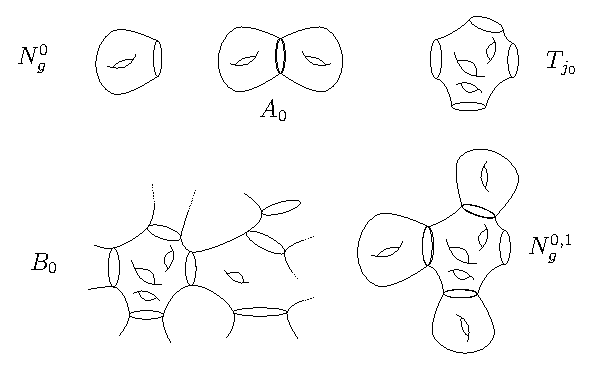
\includegraphics[width=285bp]{BuildingNg-complete.pdf}
\caption{Construction of $N_g^{0,1}$.}\label{fig:2}
\end{figure}

If $\gamma$ is a geodesic of $N_g^{0,1}$, with endpoints in the boundary, and orthogonal to the boundary, there is a dichotomy. Either it remains inside $T_{j_0}$, or it must reach the other boundary components of $T_{j_0}$. In the first case, its length must lie in $\fkG(N_g^0)$, because $T_{j_0}$ is a cover of $N_g^0$. It also cannot be a lift of $\gamma_0$ (because of our choice of~$T_{j_0}$). In the second case, the length must be at least $4\ell_0$.

We deduce that $N_g^{0,1}$ satisfies the same interesting properties as $N_g^0$ (i.e is hyperbolic, and has totally geodesic boundary isometric to $\Sigma$), and
\[
\fkG\left(N_g^{0,1}\right) \subset \fkG\left(N_g^0\right)\cup [4\ell_0,+\infty\mathclose{[}.
\]
Additionally, there are at most $m_0-1$ geodesics orthogonal to the boundary in $N_g^{0,1}$, with length exactly $2\ell_0$.

Iterating this process, we build thus a manifold $N_g^1$ with the same interesting properties as $N_g^0$, such that
\[
\fkG\left(N_g^{1}\right) \subset \left(\fkG\left(N_g^0\right)\setminus\{2\ell_0\}\right)\cup [4\ell_0,+\infty\mathclose{[}.
\]
Repeating the argument for $\ell_1$ (if $\ell_1<4\ell_0$), we build in a finite number of steps a manifold $N_g^2$ with same interesting properties as $N_g^0$, such that
\[
\fkG\left(N_g^{2}\right) \subset [4\ell_0,+\infty\mathclose{[}.
\]
By finite induction, we finally obtain a manifold $N_g^3$ with same interesting properties as $N_g^0$ such that
\[
\fkG\left(N_g^{3}\right) \subset\mathopen{]}4\kappa,+\infty\mathclose{[}.
\]
This is what we wanted to find.
\end{proof}

This closes the proof of Theorem~\ref{thm:compact-embedding-geometry}.
\end{proof}

Observe that there are examples of compact hyperbolic 4-manifolds whose $\pi_1$ is not LERF. This highlights the difficulty of the problem in higher dimensions.

Let us prove Corollary~\ref{cor:1}:

\begin{proof}[Proof of Corollary~\ref{cor:1}]
Let $(M,g)$ be an oriented Anosov 3-manifold with boundary. Then we have seen that $M$ can be embedded as a convex open set of a compact manifold $(M',g)$, with Anosov geodesic flow. According to the geometrization theorem, since $M'$ is aspherical, it must be irreducible. Additionally, there can be no $\Z^2$ in its fundamental group, so that it is actually locally homogeneous, and it must be a hyperbolic manifold, with metric $\tilde{g}$. It follows that $\Gamma=\pi_1(M)\subset \pi_1(M')\subset \PSL_2(\C)$, and we consider $M''= \Hh^3/\Gamma$. It is homeomorphic to $M$, and contains $M$ as a strictly convex subset for the metric $g$.

Let us recall an explicit conjugation between the geodesic flows. This construction is due to Morse according to~\cite{Gromov-00}, however we refer to~\cite[Appendix~B]{Guillarmou-Knieper-Lefeuvre} for detailed explanations and proofs. Working first on the universal cover, given a~vector $(x,v)\in S^\ast \Hh^3$, we can consider the endpoints $p_{\pm}$ in the boundary at infinity of the geodesic through $(x,v)$ for the metric $g$. Let ${\gamma}$ be the geodesic for $\tilde{g}$ with the same endpoints, and $H$ the horosphere based at $p_+$ through $x$, for the metric $\tilde{g}$. Then $H$ and $\gamma$ intersect at exactly one point $\gamma(t)$, and we set $h_0(x,v) = (\gamma(t),\gamma'(t))$. This map is uniformly H\"older, and equivariant under the action of $\pi_1(M')$. It also is a~semi-conjugation of the geodesic flows with a time change called ``geodesic stretch''.

If $g$ and $\tilde{g}$ are not close, it is not quite clear whether the map $h_0$ is injective or not, however Gromov observes that we may average $h_0$ along the orbits of the geodesic flow of $g$, to obtain a new map $h$; if the chosen time scale is large enough, $h$ is still equivariant, H\"older; it conjugates the geodesic flows with a new time change; crucially it is now bijective\footnote{Here we used the compactness of $M'$ to ensure that the time scale, which is chosen locally uniformly orbit wise can be chosen globally.}.


Using equivariance, $h$ descends to a homeomorphism of $S^\ast (M'')$, mapping the geodesic orbit foliation of $g$ to that of $\tilde{g}$. The group $\Gamma$ is convex co-compact if the set
\[
\Omega_{\tilde{g}} \simeq_{\tilde{g}} (\Lambda\times\Lambda\setminus\Diag \times\R)/\Gamma
\]
is compact (here $\simeq_{\tilde{g}}$ are the Hopf coordinates related to $\tilde{g}$, and $\Lambda$ is the limit set of~$\Gamma$). However, we get that $\Omega_{\tilde{g}} = h(\Omega_g)$, where naturally
\[
\Omega_{{g}} \simeq_{g} (\Lambda\times\Lambda\setminus\Diag \times\R)/\Gamma \subset S^\ast M.
\]
To close the proof, let us recall an argument to obtain a smooth strictly convex neighbourhood of the convex core in convex co-compact manifolds. It is a classical result (really an alternative definition of convex co-compactness) that $U=\partial^\infty \Hh^3 \setminus \Lambda$ is a discontinuity domain for the action of $\Gamma$, and that $M''$ is conformally compact, with compactification
\[
\bar{M''}= M'' \cup U/\Gamma.
\]
Near the boundary, one can find a smooth boundary defining function $x$, and the metric takes the form
\[
g = \frac{g_0}{x^2}, \quad x>0.
\]
Here $g_0$ is a smooth metric on $\bar{M''}= \{x\geq 0\}$. It is possible to find coordinates (see for example~\cite[Lemme~2.1.2]{Guillarmou-et-al}) such that we are in a slice situation as Section~\ref{sec:metric-extension}, and setting $t=\log (1/x)$,
\[
g = dt^2 + e^{2t}h(e^{-t}),
\]
$h$ being a metric on the slice. The second fundamental form of the slice $\{t=t_0\}$ is
\[
e^{2t}h(e^{-t}) - e^t \partial_x h(e^{-t}) \sim e^{2t} h(0) > 0.
\]
This ensures that the slice is strictly convex as $t_0\to +\infty$.
\end{proof}


Let us conclude the proof of the main theorem~\ref{thm:3D}.
\begin{proof}[Proof of Theorem~\ref{thm:3D}]
We have already embedded isometrically $M\subset N'$, so that the curvature of $N'$ satisfies:
\begin{enumerate}
\item $K \leq C_0$ globally,
\item $K \leq - \kappa^2 /2$ on $N'\setminus V$, where $V$ is the $1/\sqrt{\kappa}$ neighbourhood of $M$.
\end{enumerate}
We have seen that $C_0$ is fixed, and $\kappa$ can be taken arbitrarily large. We have also ensured that the slices are uniformly strictly convex. In the arguments below, $C>0$ will denote a constant that does not depend on the choice of $\kappa$, and that may change at every line. We will use the notations for Jacobi fields introduced in~\cite{Chen-Erchenko-Gogolev}. Let us just recall that if $J$ is a Jacobi field,
\[
\mu_J(t) = \frac{1}{2}\frac{(\| J(t) \|^2)'}{\|J(t)\|^2}.
\]
We also denote by $\partial_{\pm} \SM$ the set of vectors in $\SM$ above $\partial M$ that are entering (-) and outgoing (+). Also denote by $\Gamma_{\pm}$ the set of entering (-) (resp. outgoing (+)) vectors that are trapped in $M$ for all positive (resp. negative) time. For vectors not in $\Gamma_+$ we denote by $l_g(v)$ the time when they exit $M$.

Observe that the constant $1/C_1$ in~\cite{Chen-Erchenko-Gogolev} corresponds to our $1/\sqrt{\kappa}$. The key technical tool is the comparison~\cite[Lemma~2.8]{Chen-Erchenko-Gogolev} itself taken from Gulliver~\cite[Lemma~3]{Gulliver-75}, that we reproduce for convenience.

\begin{lemm}[{\cite[Lemma~3]{Gulliver-75}}]
Let $\gamma$ be a geodesic on a Riemannian manifold $M$ and let $J$ be a perpendicular Jacobi field along $\gamma$. Assume that $f:\R\to\R$ is integrable on bounded sets and gives an upper bound on sectional curvature as follows
\[
K\left(\sigma_{\gamma'(t), J(t)}\right) \leq f (t)
\]
for all $t$. Let $s^\ast\in\R$ and let $u$ be a solution of $u''+f u = 0$ with $u(s^\ast)= \|J(s^\ast)\|$, $u'(s^\ast)\leq \|J'(s^\ast)\|$. Assume that $u(t)>0$ for $s^\ast < t \leq s^{\ast\ast}$. Then for any $s^\ast < t \leq s^{\ast\ast}$, $J(t)\neq 0$ and
\[
\mu_J \geq u' / u.
\]
\end{lemm}

In particular, we deduce that in $N'\setminus V$, i.e the region $t>1/\sqrt{\kappa}$, where the curvature is below $-\kappa^2/2$, a Jacobi field with $\mu_J(0)> - Q$ satisfies $\mu_J(t)>(1-\epsilon)\kappa/\sqrt{2}$ for $t\gtrsim 1$, when $\kappa$ is large and $Q$ remains fixed.

In~\cite[Section~4]{Chen-Erchenko-Gogolev}, this comparison lemma is used to carefully prove the following Proposition~\ref{prop:4.1}.

\begin{prop}[{\cite[Proposition~4.1]{Chen-Erchenko-Gogolev}}]
\label{prop:4.1}
Let $(M, g)$ be a manifold with boundary. Assume that $(M, g)$ has no conjugate points and a (possibly empty) hyperbolic trapped set $\Lambda$. Then, there exists constants $Q_M > 0$ and $C_M > 0$, such that for any $v \in \partial_- \SM$ and a perpendicular Jacobi field $J$ along $\gamma_v$ with $\mu_J (0) > Q_M$, $J$ does not vanish as long as $\gamma_v$ lies in $M$. Moreover, the following properties hold:
\begin{enumerate}
\item\label{prop4.6.1} If $v \in \Gamma_-$, then $\| J(t)\|\to \infty$ as $t\to\infty$.
\item\label{prop4.6.2} If $v\in \Gamma_-$, then $\mu_J(l_g(v)>-Q_M$ and $\int_0^{l_g(v)} \mu_J(\tau)d\tau \geq C_M$.
\item\label{prop4.6.3} For any sufficiently small $\delta>0$, let $M_{-\delta}=\{x\in M\ |\ \dist_g(x,\partial M)\geq \delta\}$. Then, \eqref{prop4.6.1} and~\eqref{prop4.6.2} remain valid with the same $Q_M$ and $C_M$ if we replace $M$ with $M_\delta$.
\end{enumerate}
\end{prop}

We essentially rely on the arguments of~\cite[Section~8]{Chen-Erchenko-Gogolev}, but we have reorganized the order a bit. We will only insist on key details. The constant $Q_0$ appearing many times in~\cite[Section~8]{Chen-Erchenko-Gogolev} is the constant $Q_{\{t\leq \delta_0\}}$ of Proposition~\ref{prop:4.1} for some $\delta_0>0$ arbitrarily small. We denote it by $Q_M$ here. The following statement has no direct equivalent in~\cite{Chen-Erchenko-Gogolev} (but the arguments of proof come from several parts of Section~8 therein).

\begin{lemm}\label{lemma:our-lemma}
Let $v\in \partial_- \SM$ and $J$ be a perpendicular Jacobi field along the corresponding geodesic. If $\mu_J(0)>Q_M$, then $J$ does not vanish in positive time.
\end{lemm}


\begin{proof}
According to~\cite[Lemma~8.5]{Chen-Erchenko-Gogolev}, the time travel in the region $t\in [0,1/\sqrt{\kappa}]$ is bounded above by $C/\sqrt{\kappa}$. If $J$ a perpendicular Jacobi field along a geodesic $\gamma_v$ starting at a point $v\in \SN'$, let us assume that $v\in \partial \SM$ is entering. Then according to~\cite[Proposition~4.1]{Chen-Erchenko-Gogolev}, if $\mu_J(0) > Q_M$, either $v\in\Gamma_-$ and we are done, or $\gamma\notin \Gamma_-$. Then as $\gamma_v$ leaves $\SM$, $\mu_J(\ell(v)) > - Q_M$. Since the travel time in the collar is small and the curvature bounded above, we deduce that $\mu_J$ is at least $-2Q_M$ when $\gamma_v$ enters $\{t>1/\sqrt{\kappa}\}$. Now, in this region, the curvature is bounded above by $-\kappa^2/2$, so that applying the comparison~\cite[Lemma~2.8]{Chen-Erchenko-Gogolev}, and taking into account that the travel time inside $t>1/\sqrt{\kappa}$ must be at least $1$, if $\kappa$ is large enough, $\mu_J$ must be at least $Q_M$ again when $\gamma_v$ enters again $\SM$ (if it ever does). We can conclude by induction on the times.
\end{proof}

\begin{lemm}
$N'$ has no conjugate points.
\end{lemm}

\begin{proof}
Let us consider a nonzero Jacobi field $J$ that vanishes at some point above $N'\setminus M$. Then, using again the comparison lemma, we deduce that $\mu_J> Q_M$ as long as the geodesic remains in $\SN'\setminus \SM$, and thus cannot vanish again according to Lemma~\ref{lemma:our-lemma}.

Let us now consider a nonzero Jacobi field vanishing at some point. If the corresponding geodesic remains in $\SM$, then we are done. Otherwise consider the first time that it exits $\SM$. Then, using the argument of the proof of~\cite[Lemma~8.11]{Chen-Erchenko-Gogolev}, we must have $\mu_J> - Q_M$. Otherwise we could apply Proposition~4.1 in reversed time, and obtain a contradiction. Again by the smallness of the collar and the very negative curvature in $\{t>1/\sqrt{\kappa}\}$, if the geodesics come back again in $\SM$, we must have $\mu_J> Q_M$ at the point of entry. Then proceeding by induction as above enables us to conclude.
\end{proof}

Finally, we have to prove that the geodesic flow is Anosov. For this it suffices, according to Eberlein's theorem, to prove that no nonzero Jacobi field can be globally bounded. Since $M$ has axiom A geodesic flow and the curvature is very negative in $\{t>1/\sqrt{\kappa}\}$, this is a given for any Jacobi field along a geodesic that remains either in $\SM$ or $\SN'\setminus \SM$ for all times.

Consider a geodesic $\gamma$ entering $\SM$ at a point $v$, with a perpendicular Jacobi field $J$ satisfying $\mu_J> Q_M$ at that point. Then according to~\cite[Proposition~4.1]{Chen-Erchenko-Gogolev}, we have either $\|J\|\to+\infty$, or $\int_{\SM} \mu_J > -C_0$ before $\gamma$ exits $\SM$. Now, before the geodesic enters again (if it ever does) in $\SM$, since the curvature is so negative, using the comparison lemma again, we must have
\[
\int_{\SN\setminus \SM} \mu_J\geq (1-\epsilon) \frac{\kappa}{\sqrt{2}} - \epsilon,
\]
where $\epsilon$ tends to $0$ as $\kappa$ grows large. Here we have taken into account that the travel time must be at least $1$ above $N'\setminus M$. We also used~\cite[Proposition~4.1]{Chen-Erchenko-Gogolev}, ensuring that $\mu_J>-Q_M$ entering $\SN'\setminus \SM$.

Now, either the sequence of times when the geodesic changes component is finite, and we know directly by the comparison lemma and Proposition~4.1 that $|J|\to+\infty$, or the sequence is infinite. In that case, we observe that between two consecutive times the geodesic entered $\SM$, we have
\[
\intt \mu_J > \frac{1}{10}\kappa - C_0 > 1,
\]
so that $\|J\|\to+\infty$ also in positive time.

Let us now consider the case that as $\gamma$ enters $\SM$, $\mu_J \leq Q_M$. Then, we reverse time, and see this as a geodesic entering $\SN'\setminus \SM$ with $\mu_J \geq - Q_M$. Then the same argument as above apply, only in negative time.
\end{proof}



\begin{thebibliography}{99}
\bibitem{Agol2012}Agol, Ian The virtual Haken conjecture (with an appendix by Ian Agol, Daniel Groves and Jason Manning)., Doc. Math., Volume 18 (2013), pp. 1045-1087 | Zbl | DOI | MR
\bibitem{DoCarmo}do Carmo, Manfredo Perdigão Geometria Riemanniana, Projeto Euclides, IMPA - Instituto de Matemática Pura e Aplicada, 2015 | Zbl | MR
\bibitem{Chen-Erchenko-Gogolev}Chen, Dong; Erchenko, Alena; Gogolev, Andrey Riemannian Anosov extension and applications, J. Éc. Polytech., Math., Volume 10 (2023), pp. 945-987 | DOI | Zbl | MR | Numdam
\bibitem{Guillarmou-et-al}Djadli, Zindine; Guillarmou, Colin; Herzlich, Marc Opérateurs géométriques, invariants conformes et variétés asymptotiquement hyperboliques, Panoramas et Synthèses, 26, Société Mathématique de France, 2008 | Zbl | MR
\bibitem{Erchenko-Lefeuvre}Erchenko, Alena; Lefeuvre, Thibault Marked boundary rigidity for surfaces of Anosov type, Math. Z., Volume 306 (2024) no. 3, 36, 22 pages | DOI | Zbl | MR
\bibitem{Freitas}de Freitas, Izabella M.; Ramos, Álvaro K. Geometrization in Geometry (2022) | arXiv
\bibitem{Fujii}Fujii, Michihiko Hyperbolic 3-manifolds with totally geodesic boundary, Osaka J. Math., Volume 27 (1990) no. 3, pp. 539-553 | Zbl | MR
\bibitem{Guillarmou-Knieper-Lefeuvre}Guillarmou, Colin; Knieper, Gerhard; Lefeuvre, Thibault Geodesic stretch, pressure metric and marked length spectrum rigidity, Ergodic Theory Dyn. Syst., Volume 42 (2022) no. 3, pp. 974-1022 | DOI | Zbl | MR
\bibitem{gromov}Gromov, Mikhael L.; Lawson, Herbert B. Jr; Thurston, William P. Hyperbolic 4-manifolds and conformally flat 3-manifolds, Publ. Math., Inst. Hautes Étud. Sci., Volume 68 (1988), pp. 27-45 | DOI | Zbl | Numdam | MR
\bibitem{Gromov-00}Gromov, Mikhael L. Three remarks on geodesic dynamics and fundamental group, Enseign. Math. (2), Volume 46 (2000) no. 3-4, pp. 391-402 | Zbl | MR
\bibitem{Gulliver-75}Gulliver, Robert On the variety of manifolds without conjugate points, Trans. Am. Math. Soc., Volume 210 (1975), pp. 185-201 | DOI | Zbl | MR
\bibitem{Hatcher}Hatcher, Allen Algebraic topology, Cambridge University Press, 2002 | Zbl | MR
\bibitem{Klingenberg-1974}Klingenberg, Wilhelm Riemannian Manifolds With Geodesic Flow of Anosov Type, Ann. Math. (2), Volume 99 (1974) no. 1, pp. 1-13 | DOI | Zbl
\bibitem{Kobayashi-61}Kobayashi, Shoshichi Riemannian manifolds without conjugate points, Ann. Mat. Pura Appl. (4), Volume 53 (1961), pp. 149-155 | DOI | Zbl | MR
\bibitem{Milnor}Milnor, John W. A Unique Decomposition Theorem for 3-Manifolds, Am. J. Math., Volume 84 (1962) no. 1, pp. 1-7 | DOI | Zbl | MR
\bibitem{convex-plumbing}Martelli, Bruno; Riolo, Stefano; Slavich, Leone Convex plumbings in closed hyperbolic 4-manifolds, Geom. Dedicata, Volume 212 (2021), pp. 243-259 | DOI | Zbl
\end{thebibliography}
\end{document}
